% $Id: fem.tex,v 1.12 2001-07-18 09:09:51 geuzaine Exp $

% ---------------------------------------------------------------------------
\part{Introduction}
% ---------------------------------------------------------------------------

\begin{slide}

\slidepagestyle{none}

\begin{center}
\bigtitle{Introduction --- finite element methods}
\ifnum\fulltitle=1\par\bigskip\bigskip
\mediumtitle{Christophe Geuzaine}\\
\bigskip
\smalltitle{Department of Electrical Engineering}\\
\smalltitle{Montefiore Institute B28, Sart Tilman Campus}\\
\smalltitle{University of Li�ge}\\
\smalltitle{B-4000 Li�ge (BELGIUM)}
\fi
\end{center}

\end{slide}

% ---------------------------------------------------------------------------

\chapter{Coupled electromagnetic problems?}

\begin{slide}

Maxwell's equations, coupled with...

\begin{slideitemize}
\item Electric and electronic \emph{circuits} (power electronic supplies)
\item \emph{Mechanical} phenomena (force calculation, magnetostriction,
piezoelectricity, noise and vibrations)
\item \emph{Thermal} phenomena (thermal losses, induction heating, dielectric heating)
\item \emph{Fluid} dynamics (charged particles, magnetohydrodynamics)
\end{slideitemize}

\end{slide}

% ---------------------------------------------------------------------------

\chapter{Computational methods?}

\begin{slide}

\begin{slideitemize}
\item \emph{Analytic} models are difficult/impossible to apply to complex/coupled problems
\item \emph{Performance} (both floating point and visualization) of low end PCs is
exploding
\item Basic \emph{theory} of classic numerical methods (finite differences,
finite volumes, finite elements, integral methods) is well-known, and current
developments don't change the fundamental principles anymore
\end{slideitemize}

\end{slide}

% ---------------------------------------------------------------------------

\chapter{Finite element method (FEM)}

\begin{slide}

\begin{slideitemize}
\item The 1960s for mechanical problems (very large \emph{application range}
since the 1980s)
\item Strong \emph{mathematical foundations} (convergence, unicity)
\item Generalizations/re-interpretations (vanishing boundaries between finite
differences, finite elements and finite volumes, ...) call for a
\emph{single software implementation}
\end{slideitemize}

But FEM is not the magic/universal tool:
\begin{slideitemize}
\item Many conflicting/\emph{antinomic} issues (continuous vs. discontinuous
interpolation, conforming vs. non-conforming meshes, implicit vs. explicit
time integration, ...)
\item Generality has always an impact on \emph{efficiency}
\end{slideitemize}

\end{slide}

\begin{slide}

Based on a double \emph{discretization}:
\begin{slideitemize}
\item ``Replace'' the function spaces to which the fields belong (e.g.\
$\Hone{\Omega}$, $\Hcurl{\Omega}$, $\Hdiv{\Omega}$ or $\Ltwo{\Omega}$) by
\emph{finite dimensional subspaces}
\item ``Replace'' the domains on which these subspaces are defined by a
union of elementary geometrical elements of simple shapes (a ``\emph{mesh}''
or ``grid'')
\end{slideitemize}

\bigskip

\mybox{colbox}{0.98\textwidth}{
\begin{center}
FEM\\ $\Updownarrow$\\ the finite dimensional subspaces are built so that
their bases are \emph{piece-wise} defined on the mesh
\end{center}
}

\end{slide}

\begin{slide}

One way to obtain a consistent Galerkin FEM formulation:
\begin{slideitemize}
\item Write a \emph{weak formulation} of the problem:

\begin{equation*}
\begin{cases}
L u = f \text{ in } \Omega \\
B u = g \text{ in } \Gamma 
\end{cases}
\Rightarrow\quad
\ivol[_\Omega]{u}{L^* v} - 
\ivol[_\Omega]{f}{v} + 
\int\limits_\Gamma Q_g(v) \, ds , 
\quad\forall v \in V(\Omega) 
\end{equation*}

% $L$ is a differential operator of order $n$ defined on $\Omega$
% 
% L^* is the adjoint of L:
%
% \ivol[_\Omega]{L u}{v} - \ivol[_\Omega]{u}{L^* v} = \int\limits_\Gamma Q(u,v) ds ,
%
% $Q$ is a bilinear function of $u$ and $v$ and in their derivatives up
% to the order $n-1$
%
% $Q_g$ is a linear form in $v$ which depends of $g$

\item Discretize with \emph{Whitney/mixed} elements $w_i$:
\begin{equation*}
\bar{u}, \bar{v} \in W(\Omega) , \quad
W(\Omega) = \text{span}\{w_i\} , \quad
W(\Omega) \subset V(\Omega)
\end{equation*}

% \bar{u} = \sum_{i} u_i w_i 

\end{slideitemize}

\end{slide}

\begin{slide}

\begin{slideitemize}
\item ``\emph{Nodal}'' elements for ``0-forms'' (\emph{continuous} scalar
fields like scalar potentials, temperature, pressure, ...)

\item ``\emph{Edge}'' elements for ``1-forms'' (vector fields with
\emph{continuous tangential components} across material interfaces, like
electric and magnetic fields, magnetic vector potential, ...)

\item ``\emph{Facet}'' elements for ``2-forms'' (vector fields with
\emph{continuous normal components} across material interfaces, like
magnetic flux density, current density, ...)

\item ``\emph{Volume}'' elements for ``3-forms'' (\emph{piece-wise
continuous} scalar fields like charge density, heat source density, ...)

\end{slideitemize}

\end{slide}

% ---------------------------------------------------------------------------

\chapter{Controlling the error}

\begin{slide}

\emph{Error} on the solution of a discrete formulation:
\begin{slideitemize}
\item 
\emph{Hypotheses} in the continuous models (e.g.\ constitutive laws) 
\item 
\emph{Discretization} of the continuous model (finite dimensional spaces):
\begin{itemize}
\item 
Discretizing the \emph{geometry} (idealized geometry, meshed with a finite
number of elementary elements)
\item
Discretizing the \emph{fields} (locally approximated by polynomials of
finite order)
\end{itemize}
\end{slideitemize}

\end{slide}

\begin{slide}

\emph{Adaptation}: foresee/control the discretization error. Possible if
\begin{slideitemize}
\item
Knowledge of asymptotic \emph{error convergence}
\item
Availability of an error \emph{approximation} (if the exact value is known,
so is the exact solution!)
% the exact solution is also known!)
\end{slideitemize}

Goal: generate the best discrete function space possible 

Constraint: size of the function space or discretization error

Solution: modify (if possible, locally) the interpolation order
(\emph{$p$-refinement}) or the size of geometrical elements
(\emph{$h$-refinement})

\end{slide}

% ---------------------------------------------------------------------------

\chapter{Local and global errors}

\begin{slide}

If $u$ and $u'$ are the exact and approximate solutions on $\Omega$:
\begin{slideitemize}
\item
Elementary and global \emph{absolute} errors $e_i$ and $e$
\begin{equation*}
e_i^2 = \ivol[_{K_i}]{u'-u}{u'-u} \quad\text{and}\quad
e^2   = \ivol[_\Omega]{u'-u}{u'-u}
\end{equation*}
\item
Elementary and global \emph{relative} errors
\begin{equation*}
\varepsilon_i^2 = e_i^2 / n^2 \quad\text{and}\quad
\varepsilon^2   = e^2 / n^2 = \sum_{i=1}^N \varepsilon_i^2
\end{equation*}
\begin{equation*}
n^2 = \ivol[_\Omega]{u'+u}{u'+u}
\end{equation*}
\end{slideitemize}

\end{slide}

% ---------------------------------------------------------------------------

\chapter{Error convergence for elliptic problems}

\begin{slide}

\begin{slideitemize}
\item If $h_i$ and $p_i$ measure the size and polynomial degree of element
$K_i$: 
\begin{equation*}
\varepsilon_i = \Order\Big( \frac{1}{p_i} h_i^{\min(p_i,\gamma)} \Big) 
\end{equation*}
($\gamma$ depends on singularities of $u$)
\item
If \emph{uniform} error distribution (or no singularities):
\begin{equation*}
\varepsilon_i = \Order\Big( \frac{1}{p_i} h_i^{p_i} \Big) 
\end{equation*}
\end{slideitemize}

\end{slide}

% ---------------------------------------------------------------------------

\chapter{Error estimates through dual solutions}

\begin{slide}

\begin{slideitemize}
\item
Two \emph{dual} formulations, each being conform on one side of a Tonti diagram
\item
Error estimated through \emph{non fulfillment of the constitutive
relations}. For example:
\begin{equation*}
\varepsilon_i^\mu       = \frac{\Norm{\vec{b}-\mu\vec{h}}_{K_i}} 
                                {\Norm{\vec{b}+\mu\vec{h}}_\Omega} ,\quad
\varepsilon_i^\epsilon  = \frac{\Norm{\vec{d}-\epsilon\vec{e}}_{K_i}}
                                {\Norm{\vec{d}+\epsilon\vec{e}}_\Omega} \quad\text{and}\quad
\varepsilon_i^\sigma    = \frac{\Norm{\vec{j}-\sigma\vec{e}}_{K_i}}
                                {\Norm{\vec{j}+\sigma\vec{e}}_\Omega}
\end{equation*}
\item
\emph{Hypercirle theorem} implies upper bounds to the exact error for non
dissipative systems.
\item
For other systems, if mesh size sufficiently small, ...
\end{slideitemize}

\end{slide}

\begin{slide}

Example: convergence of global quantities (inductance and resistance) for
dual formulations

\centerline{
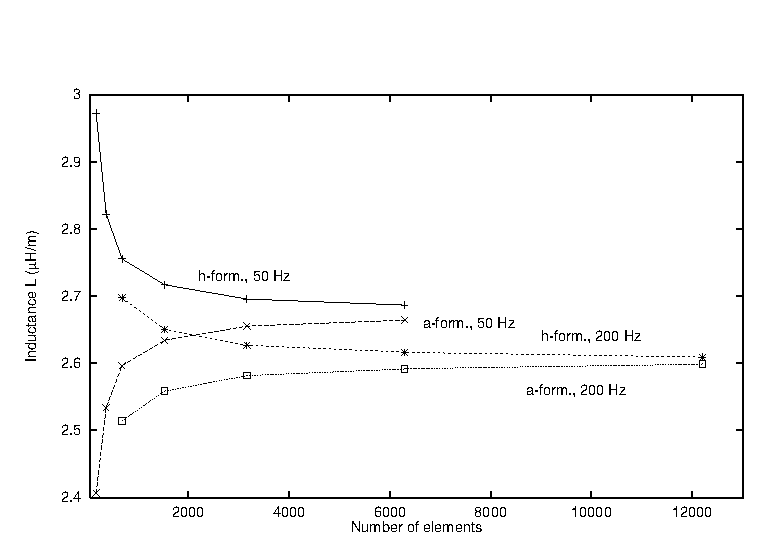
\includegraphics[width=11\semcm]{fig/IndL}
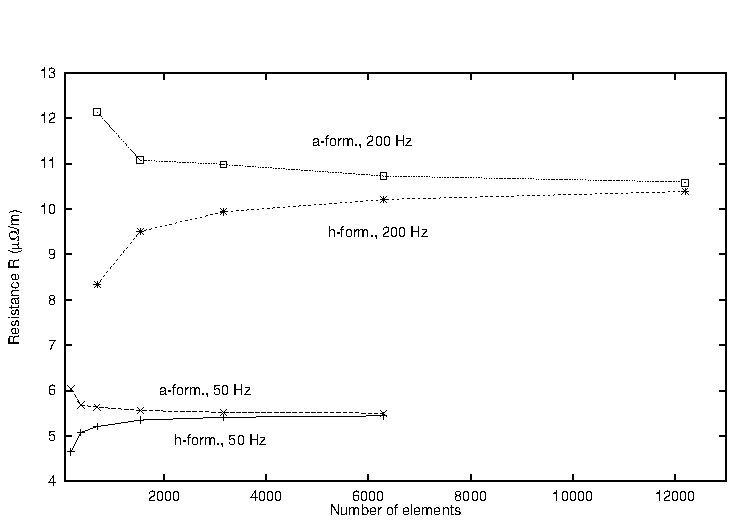
\includegraphics[width=11\semcm]{fig/IndR}
}

\end{slide}

\begin{slide}
\emph{Deterministic optimization of the global spaces}: minimize the number of
unknowns, while respecting a prescribed global error $\varepsilon_0$
\begin{equation*}
\min_{h_i',p_i'} \sum_{i=1}^N {p_i'}^3 (h_i/h_i')^3 
\quad\text{with}\quad
\varepsilon_0^2 =
\sum_{i=1}^N \varepsilon_i^2 \,
 \frac{p_i^2 \, {h_i'}^{2 p_i'}}{{p_i'}^2 \, h_i^{2 p_i}}
\end{equation*}

\begin{enumerate}
\item 
solve on $\mathcal{M}$;
\item 
create $\mathcal{M}'$ by \emph{$h$-adaptation} with a global constraint
$\alpha\varepsilon''$ ($\alpha>1$);
\item 
solve on $\mathcal{M}'$;
\item 
create $M''$ by \emph{$p$-adaptation} with the global constraint
$\varepsilon''$. Since the uniform error distribution was achieved on
$\mathcal{M}'$, this leads to the ideal convergence rate;
\item
solve on $\mathcal{M}''$.
\end{enumerate}
\end{slide}

\begin{slide}

Disadvantages of the dual approach:
\begin{slideitemize}
\item
Both dual formulations have to be solved (\emph{cost!})
\item
Implementation of one formulations usually (much) \emph{harder} than the
other
\end{slideitemize}

Solutions?
\begin{slideitemize}
\item
Projection techniques
\item
Generalize the software tools to tackle various formulations easily
\end{slideitemize}

\end{slide}
